\documentclass[../main.tex]{subfiles}
\begin{document}


\section{Data Visualisation: A Brief History}\label{brief-history}

Data visualisation, which can be thought of as the practice of
representing information in a visual modality \cite{hinterberger_2009},
is difficult to concretely define, classify, and categorise. With the
primacy of vision with regards to our interactions with and
interpretations of the world around us, data visualisation may be
thought of as an extension of art and the written word. Both art and
writing are ancient phenomena, with evidence for the former being found
in the prehistoric period some 66,000 years ago \cite{standish_2025},
and evidence for the latter emerging as Mesopotamian cuneiform around
3200 B.C.E \cite{schmandt_2014}. Broadly, the literature agrees that art
emerged prior to the written word; this speaks volumes of the human
instinct to represent our thoughts, feelings, emotions, and that which
we interact with in the world around us pictorially. This instinct has
not waned, and modern computing makes it easier than ever for those of
us with no technical or artistic skills to create graphics and
visualisations that \emph{tell stories} about our data in ways which are
both beautiful and practical.

When, then, should we consider to be the emergence of data visualisation
as a human practice? Schmandt-Besserat
\cite{schmandt_1978, schmandt_2014} considers clay counting tokens to be
the direct precursor of the written word. While the evidence for this
link is controversial \cite{robson_2007}, the existence of such tokens
is not. With each shape of token representing a certain amount of a
certain good (measures of grain, jars of oil, etc.), this system could
be considered a very early, very simple form of data visualisation (or
physicalisation \cite{jansen_2015}). Similarly, there is limited
evidence of prehistoric cartographic drawings \cite{muhly_1978}, which
may also be considered a form of, or related to, data visualisation.
While I am not asserting that data visualisation is older than writing,
or that ancient map drawings are equivalent to modern graphics, the
existence of these representations emphasises the attractive convenience
that symbols and signs represent for humans; making sense of our world
and the relationships therein is often easier through pictures as
opposed to words and numbers, a principle which I consider key for this
thesis.

Note: much of the rest of this section is heavily inspired by Michael
Friendly's \emph{A Brief History of Data Visualization}
\cite{friendly_2008}.

Moving on, then, to the kind of pictorial representation that modern
students and scientists would firmly recognise as a ``data
visualisation''. Tufte and Graves-Morris, in 1983's seminal \emph{The
Visual Display of Quantitative Information} \cite{tufte_1983}, describe
an unattributed time series illustration from the 10th or 11th century,
itself described by Funkhouser in 1936 \cite{funkhouser_1936} as being
discovered by Sigmund Günther in 1877. This illustration is included
here in Figure~\ref{fig-early-time-series}.

\begin{figure}

\centering{

\includegraphics[width=\textwidth]{../supplied_graphics/tufte_1983.png}

}

\caption{\label{fig-early-time-series}Reproduced in Tufte and
Graves-Morris, 1983 \cite{tufte_1983} from Funkhouser, 1936
\cite{funkhouser_1936}.}

\end{figure}%

This illustration purports to show the movements of planetary bodies as
a function of time, although Funkhouser considered it little more than a
``schematic diagram\ldots for illustrative purposes''
\cite{funkhouser_1936}. Regardless, the recognisable grid lines and
sinusoidal variation in the curves are ideas that would not appear again
for another 600-700 years, after which they would become mainstream
visualisation techniques. In the mid-14th century, French philosopher
Nicole Oresme demonstrated an understanding of graphing by plotting
proto-bar charts, and by the 16th century, advances in cartography,
photography, and mathematics laid the ground for an explosion in data
visualisation.

The 17th century saw the birth of geometry and coordinate systems, error
measurement, probability, and demographic statistics. With these
scientific advancements came the advancements in data visualisation
needed to communicate these concepts. For example, in 1626, Scheiner
used what Tufte would later term the ``principle of small multiples''
\cite{tufte_1983} to illustrate how configurations of sunspots change
over time (see Figure~\ref{fig-sunspots}).

\begin{figure}

\centering{

\includegraphics[width=\textwidth]{../supplied_graphics/sunspots.png}

}

\caption{\label{fig-sunspots}placeholder}

\end{figure}%

\begin{figure}

\centering{

\includegraphics[width=\textwidth]{../supplied_graphics/snow_cholera.jpg}

}

\caption{\label{fig-cholera}John Snow's (1854) map of cholera cases in
Soho, London. Using this data visualisation, Snow was able to
demonstrate a link between cholera cases and a contaminated water
supply.}

\end{figure}%

\begin{figure}

\centering{

\includegraphics[width=\textwidth]{../supplied_graphics/minard_napoleon.jpg}

}

\caption{\label{fig-napoleon}Charles Joseph Minard's (1869) flow diagram
of Napoleon's botched invasion of Russia in 1812-1813. This diagram
shows Napoleon's advance and retreat on Moscow. The width of the orange
and black columns encodes the size of the Grande Armée. The temperature
scale on the lower portion of the graph illustrates the weather
conditions during the retreat, with a freezing Russian winter causing
high rates of attrition.}

\end{figure}%

\begin{figure}

\centering{

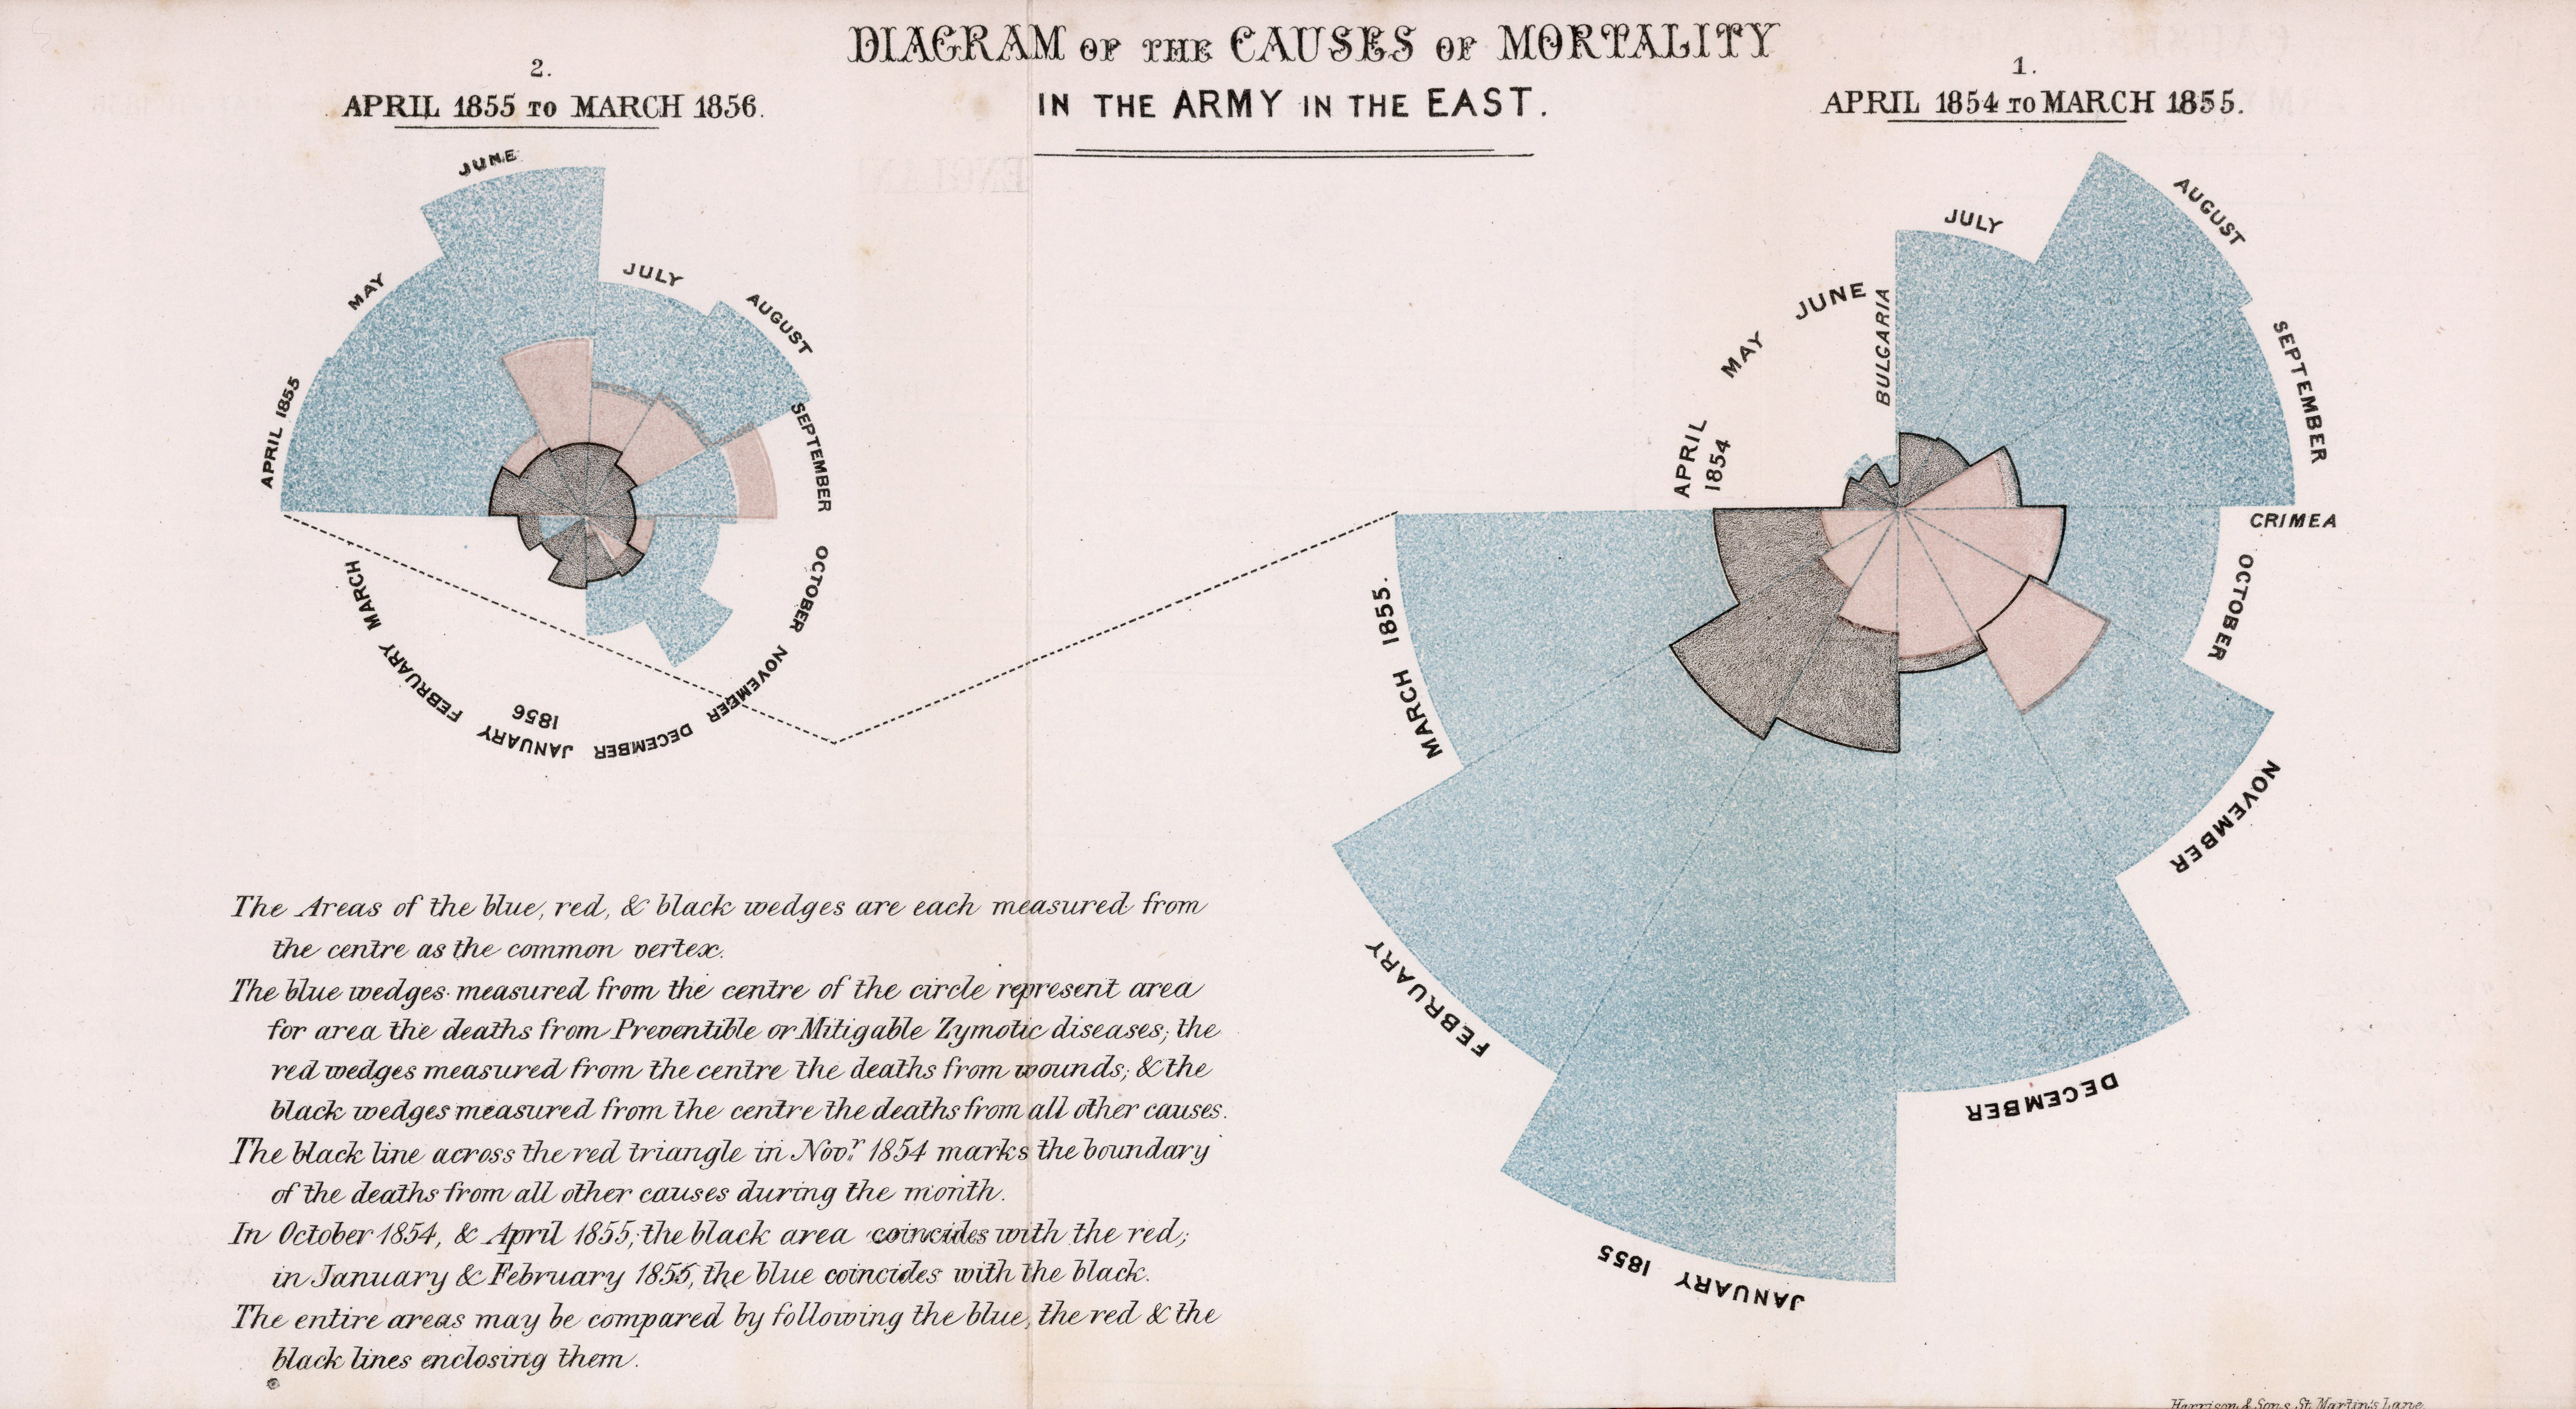
\includegraphics[width=\textwidth]{../supplied_graphics/nightingale-rose.jpg}

}

\caption{\label{fig-nightingale}Florence Nightingale's (1858) polar area
chart illustrates the causes for mortality among British soldiers during
the Crimean War. Data visualisations of this type were used to
illustrate that in reality, more British soldiers died from preventable
disease than were killed by the enemy, and were used as part of a
campaign to improve sanitation among soldiers.}

\end{figure}%

The latter half of the 19th century, the so-called ``Golden Age of
Statistical Graphics'' \cite{friendly_2008} saw the rise of forms of
data visualisation that begin to look remarkably similar to the graphs
and informatics seen in mass media and scientific publications today.
The most notable examples of these are John Snow's cholera map, which
was able to link the incidence of cholera to a contaminated water pump
in London (Figure~\ref{fig-cholera}), Charles Joseph Minard's flow chart
of the Napoleonic invasion of Russia (Figure~\ref{fig-napoleon}), and
Florence Nightingale's rose diagrams (polar area charts in the modern
parlance, see Figure~\ref{fig-nightingale}). In each of these graphs,
visualisation is used with different intent. In John Snow's cholera map,
visualisation was used to track cases of a deadly disease, and
facilitated a novel linkage between cholera and contaminated drinking
water. In Charles Joseph Minard's flow chart of Napoleon's failed 1812
invasion of Russia, a total of six variables are displayed to tell the
data story, allowing the viewer to appreciate the movements of the
Grande Armée, it's diminishing size owing to attrition, and the freezing
temperatures that largely caused that attrition. Florence Nightingale's
polar area chart depicts the causes of mortality amongst British troops
in the Crimean War; charts such as this were used to successfully
campaign for better sanitation in hospitals and the front lines.

In all of these visualisations, data is used to accentuate storytelling.
In some cases, this may lead to critical discoveries that save lives,
and in others, it may simply facilitate a greater understanding and
appreciation of the data. In either case, visualisation is used
effectively to appeal to our affinity for visual storytelling.

An appetite for precision defined the approach to statistical thinking,
and by extension, data visualisation, in the first half of the 20th
century. Statistical graphics finally became mainstream, and were
implemented in curricula and used in government, commerce, and finance.
This period also marks the beginning of graphical methods being used to
generate new scientific insights, a trend which would only accelerate
throughout the next century. The most prominent example of this is Henry
Moseley's (1913) discovery of the concept of atomic number
\cite{moseley_1913}, which I will discuss in greater detail in Section
\ref{history-corr-viz}.

Significant developments in the latter half of the 20th century laid the
final brick in the foundations of what would become the modern data
visualisation landscape. John W. Tukey's \emph{The Future of Data
Analysis} \cite{tukey_1962} proposed a separation between data analysis
and mathematical statistics. This seminal work would become hugely
influential, and Tukey would go on to invent a great number of
analysis-driven data visualisations, including stem-leaf plots and box
plots, both of which are now commonplace in software packages and
statistics education. In 1967, Jacques Bertin \cite{bertin_1967}
published \emph{Sémiologie graphique} (\emph{Semiology of Graphics}),
organising the perceptual elements of data visualisations according to
their features and their relationships to the underlying data; this work
would be influential for Leland Wilkinson's \emph{Grammar of Graphics}
\cite{wilkinson_1999}, which in turn influenced the \texttt{ggplot2}
package \cite{wickham_2016} that is used extensively in this thesis.

Since then, both the practice and study of data visualisation have
become thoroughly mainstream. Students are taught to visualise data
early on, and the propagation of both software and powerful computing
hardware have brought advanced techniques, such as high dimensional
visualisation and massive datasets, into the home. To summarise the
timeline of developments in data visualisation over the last 500 years,
I include a rug and density plot from Friendly (2008)
\cite{friendly_2008} in Figure~\ref{fig-rug-density}.

\begin{figure}

\centering{

\includegraphics[width=\textwidth]{../supplied_graphics/rug_density.png}

}

\caption{\label{fig-rug-density}Major milestones in the development of
data visualisation illustrated using a rug plot and density estimate.
This figure is taken from Friendly (2008) \cite{friendly_2008}.}

\end{figure}%

Recounting a full and detailed history of the practice and study of data
visualisation would require much more than a single thesis, and has been
done to a very high standard elsewhere
\cite{friendly_2008, friendly_2021}. Given that this thesis is focused
on the perception of correlation in scatterplots, the remainder of the
chapter is primarily limited to discussions of relatedness, correlation,
and scatterplot visualisations.

\section{Relatedness \& Correlation}\label{relatedness-and-correlation}

Very early piloting (detailed in Section
\ref{general-methods-adjusting-opacity}, \chap{chap:adjusting_opacity})
revealed that while people understood the concept of correlation, they
were unsure as to what different degrees of correlation looked like. To
address this, training was included in experiments 1 to 4. For the same
reason, correlation was operationalised as \emph{Strength of
Relatedness} in experiment 5. To make my research accessible, I start
from here; two (or more) things are related if a change in one is
associated with a change in the other(s). In reality, however, the data
visualisation under investigation, scatterplots, do not visualise
relatedness, but correlation. Correlation refers to a specific
statistical relationship, which I explore from first principles below.

Francis Galton was the first to formally introduce the concept of
\emph{co-relation} in 1888 \cite{galton_1888}. He derived a definition
of correlation as a by-product of his invention of statistical
regression, first describing this new property by way of anthropometric
data relating to the measurement of different parts of the body. Early
in this brief, but significant, paper, Galton posits a basic definition
of correlation:

\begin{quotation}
  ``Two variable organs [of the body] are said to be co-related when the variation of the one is accompanied on the average by more or less variation of the other, and in the same direction.''
\end{quotation}

Measuring a variety of anatomical distances, including head lengths and
heights of a range of ``not wholly fully-grown'' males, Galton first
provides medians and semi-interquartile ranges as a measure of error.
Plotting the semi-interquartile ranges (Q-units) of two variables
against each other and calculating the slope of the line allowed Galton
to devise a new, unitless measure of co-relatedness, which he termed r.
This has since been lauded as a prime example of a mathematical
discovery made based on observed data. This method is imprecise, as it
requires intuition of a line-of-best-fit based on a hand drawn plot, but
is credited as the first full conceptual definition of a measure of
correlation. It should be noted that Galton did not conceive of negative
correlation at this point. Galton's work did not take place in
isolation, however, and the preceding 60 years featured famous names,
such as Gauss and Darwin, dancing around the idea of correlation without
recognising its importance; Lee Rodgers \& Nicewander (1988)
\cite{lee_1988} provide an excellent overview of this period.

Building on Galton's groundbreaking work, his younger, more
mathematically-minded student, Karl Pearson, developed the Pearson
Product-Moment correlation in 1895 \cite{lee_1988} based on initial
formulae by Bravais (1844) \cite{bravais_1844}. This measure has been
remarkably persistent, remaining unchanged for well over a century. In
fact, many other measures of correlation, such as Spearman's \(\rho\),
the point-biserial correlation, and the \(\phi\) coefficient are
actually special cases of Pearson's \emph{r} applied to different types
of data \cite{henrysson_1971}; such is the dominance of the measure.
Equation 2.1 defines Pearson's \emph{r}:

\begin{equation}
  r = \frac{\sum_{i=1}^{n} (x_i - \bar{x})(y_i - \bar{y})}{\sqrt{\sum_{i=1}^{n} (x_i - \bar{x})^2 \sum_{i=1}^{n} (y_i - \bar{y})^2}}
\end{equation}

In this equation, \(\bar{x}\) and \(\bar{y}\) are the means of each
variable. \(x_i\) and \(x_i\) are the individual values of each variable
in question. In the numerator, the sum of the products of the difference
between each value of \(x\) and \(y\) is found; this value represents
the degree of deviation of all points from the regression line. Then, in
the denominator, this value is divided by the magnitude of the sum of
the product of said deviations; squaring and finding the square root of
these values provides the unsigned magnitude. In statistical language,
Pearson's \emph{r} finds the covariance of two variables, then divides
this values by the product of both variables' standard deviations.
Completing this calculation provides a measure of the overall distance
between the observed values and a fitted least squares regression line,
and provides a single value of \emph{r} that describes how strongly
related two variables are.

\section{Visualising Correlation}\label{visualising-correlation}

Of course, while mathematically sound, a single value provides no
information about the distribution of variables from which it was
derived. To do this, the data must be examined visually. Here arises a
parallel; in much the same way as Francis Galton used a
proto-scatterplot to formulate his definition of correlation, so must
data visualisation be used to tell the story behind a value of Pearson's
\emph{r}. The need for visualisation is most viscerally illustrated by
Anscombe's quartet \cite{anscombe_1973}, which is recreated in
Figure~\ref{fig-anscombe} using a dataset from the \texttt{datasets}
core package \cite{r_core} in R.

\begin{figure}

\centering{

\includegraphics[width=\textwidth]{2_related_work_files/figure-latex/fig-anscombe-1.pdf}

}

\caption{\label{fig-anscombe}Anscombe's quartet \cite{anscombe_1973}.
Each scatterplot depics datasets with identical means (\(x\) = 9, \(y\)
= 7.5), regression coefficients (\(y\) on \(x\) = 0.5), standard errors
(0.118), and Pearson's \emph{r} values (≈ 0.816).}

\end{figure}%

Anscombe's quartet \cite{anscombe_1973} describes four simple datasets
that are identical with regards to a range of statistical measures. They
feature the same number of observations, the same means, regression
coefficients, regression line equations, sums of squares, estimated
standard errors, and correlation coefficients. A simple examination of
these statistics would lead to the conclusion that the datasets are
almost identical; in reality, there are significant differences between
them that can only be seen via visualisation.

In this thesis, the primary concern is correlation and the ways in which
people interpret it from scatterplots. The remainder of this section
examines the history and current landscape of correlation
visualisations; starting with Galton's scatterplot precursors, I then go
on to discuss the development of the familiar modern scatterplot through
the examination of a number of impressive use cases. Following that, I
review the current landscape of correlation visualisation, including the
more recent use of other, non-scatterplot graphs.

\subsection{History}\label{history-corr-viz}

As mentioned in Section \ref{relatedness-and-correlation}, Francis
Galton based his initial formulation of the correlation coefficient on
hand-drawn plots of the semi-interquartile ranges of two variables.
Figure~\ref{fig-galton-hand-plot} contains a negative scan of Galton's
original plot, along with a modern recreation using \texttt{ggplot2}.

\begin{figure}

\centering{

\includegraphics[width=\textwidth]{2_related_work_files/figure-latex/fig-galton-hand-plot-1.pdf}

}

\caption{\label{fig-galton-hand-plot}Francis Galton's original plot
comparing the semi-interquartile ranges of stature (height) and cubit
(forearm length). The plot has been recreated using \texttt{ggplot2} on
the right.}

\end{figure}%

Despite the importance of graphics like these for Francis Galton's
discovery of regression, statistical correlation, and the relationship
between these and the bivariate density function \cite{friendly_2005}, a
more true example of a scatterplot can be found in much earlier work on
the orbits of twin starts by John F. W. Herschel \cite{herschel_1833}.
Unfortunately, this scatterplot was never printed in Herschel's 1833
manuscript, however can be inferred thanks to a detailed description of
both the figure and the logic behind it. In short, Herschel wished to
figure out the orbits of binary star systems by using (often imprecise)
astronomical measurements of certain angles and distances made over a
long period of time. It is the imprecision in measurement which
necessitated data visualisation, as precise measurements would would
allow common astronomical principles to provide precise solutions. First
specifying the axes, angles of position (\(y\)) and data of observation
(\(x\)), and grid lines, Herschel then describes plotting points and
drawing, by hand, a line-of-best-fit. A particularly enlightening quote,
with original emphasis, is reproduced below:

\begin{quotation}
    ``Our next step, then, must be to draw, by the mere judgement of the eye, and with
a free but careful hand, not \textit{through}, but \textit{among} them, a curve presenting as few
and slight departures from them as possible, consistently with this character of 
large and graceful sinuosity, which must be preserved at all hazards...''
\end{quotation}

From this smoothed-by-eye line, Herschel was able to calculate the
parameters that determined the rotation of the \(\gamma\)Virginis
system. Herschel beat out Galton by more than 50 years to claim the
first scatterplot, in a remarkable feat of using graphing to solve an
astronomical problem. Just a few decades after Galton had discovered the
concept of correlation, yet another astronomical example of a
scatterplot can be found in the Hertzsprung-Russell diagram, created
independently by Ejnar Hertzprung and Henry Norris Russell in 1911-1913
\cite{montmerle_2011}. This type of scatterplot, which still sees use in
modern astronomy, plots stellar luminosity against colour (temperature).
I have plotted an HR diagram in Figure~\ref{fig-HR-plot} using the HYG
database \footnote{https://www.astronexus.com/projects/hyg}.

\begin{figure}

\centering{

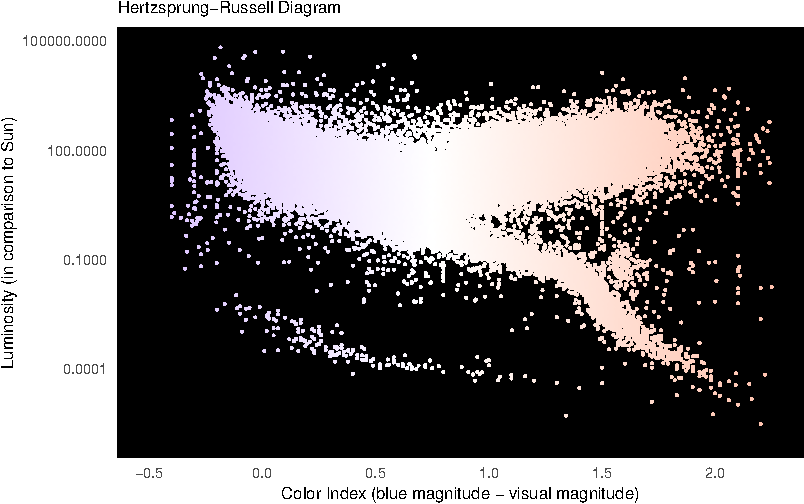
\includegraphics[width=\textwidth]{2_related_work_files/figure-latex/fig-HR-plot-1.pdf}

}

\caption{\label{fig-HR-plot}Hertzsprung-Russell diagram of colour index
against stellar luminosity. The code for this plot was taken from John
Russell's (no relation) blog \cite{russell_2025}.}

\end{figure}%

The clear band that can be seen in Figure~\ref{fig-HR-plot} from
top-left to bottom right are ``main sequence'' stars. It was only by
visualisation that astronomers were able to determine that there were
laws that govern the formation and evolution of stars. Spence and
Garrison \cite{spence_1993} conducted a detailed analysis of the history
and development of HR diagrams, and conclude that they represent a
``shining example of the power of graphic display''. Again, it was the
ability of the data visualisation to facilitate pattern recognition in
its human viewers that was so crucial to its (continuing) success.

While this section has not been an exhaustive list of every scatterplot
and scatterplot-alike that has prominently featured in scientific
publishing since Herschel's initial description and Galton's initial
formulation of correlation, I hope that I have conveyed the importance
of this visualisation type. As we will see in Section
\ref{present-landscape-corr-viz}, the landscape of correlation
visualisation is now much broader, however the humble scatterplot still
remains a crucial part of the visualisers toolbox. From its origins as a
way of inferring astronomical relationships, to its use in the discovery
of correlation, the standard scatterplot remains largely unchanged to
this day; this thesis charts the development of a new type of
scatterplot that draws on key elements of human perception to increase
its utility in correlation visualisation, however it is important to pay
homage to the history of the visualisation as an ever-present lab mate
to those able to use graphing to solve scientific problems.

\subsection{Present Landscape}\label{present-landscape-corr-viz}

\subsection{Scatterplots}\label{scatterplots-corr-viz}

\section{Correlation Perception}\label{corr-percept-related-work}

\section{Correlation Cognition}\label{corr-cognition}

\section{Underestimation: What's Really Going
On?}\label{underestimation-whats-going-on}

\section{Underestimation: Potential
Consequences}\label{underestimation-consequences}

\section{Data Visualisation Literacy}\label{graph-literacy-related-work}

\section{Objectives and Contributions}\label{objectives-contributions}




\end{document}
